\section{Linear Programming}

\subsection{Problem №1}
The company’s production facilities are such that if we devote the entire production to headphones covers, we can produce 5000 of them in one day. If we devote the entire production to phone covers or laptop covers, we can produce 4000 or 2000 of them in one day.

The production schedule is one week (6 working days), and the week’s production must be stored before distribution. Storing 1000 headphones covers (packaging included) takes up 30 cubic feet of space. Storing 1000 phone covers (packaging included) takes up 50 cubic feet of space, and storing 1000 laptop covers (packaging included) takes up 220 cubic feet of space. The total storage space available is 1500 cubic feet.

Due to commercial agreements with Random Corp has to deliver at least 4500 headphones covers and 3000 laptop covers per week in order to strengthen the product’s diffusion.

The marketing department estimates that the weekly demand for headphones covers, phone, and laptop covers does not exceed 9000 and 14000, and 7000 units, therefore the company does not want to produce more than these amounts for headphones, phone, and laptop covers.

Finally, the net profit per each headphones cover, phone cover, and laptop cover is 5, 7 and 12 \$, respectively.

The aim is to determine a weekly production schedule that maximizes the total net profit.

\begin{enumerate}
    \item[a.]  Write a Linear Programming formulation for the problem. Use following variables:
    $y_1, y_2, y_3$ - number of covers for headpnones, phones and laptops produced per week.
    \item[b.] Finf the solution to the problem using PyOMO.
\end{enumerate}

\underline{\textbf{Solution:}}


\begin{equation*}
    \begin{bmatrix} 5, 7, 12 \end{bmatrix} 
    \begin{bmatrix}
    y_1 \\
    y_2 \\
    y_3
    \end{bmatrix}  \rightarrow \max_{y \in \mathds{R}^3}
\end{equation*}

\begin{equation*}
    \begin{gathered}
        s.t. \left(y_1 \frac{30}{1000} + y_2 \frac{50}{1000} + y_3 \frac{220}{1000} \right) \leq 1500 \\
        4500 \leq y_1 \leq 9000 \\
        0 \leq y_2 \leq 14000 \\
        3000 \leq y_3 \leq 7000 \\
        \frac{y_1}{5000} + \frac{y_2}{4000} + \frac{y_3}{2000} \leq 6
    \end{gathered}
\end{equation*}

Let's rewrite this problem in terms of x: $y_1 = x_1 + 4500$, $y_2 = x_2$, $y_3 = x_3 + 3000$.

\begin{equation*}
    \begin{bmatrix} 5, 7, 12 \end{bmatrix} 
    \begin{bmatrix}
    x_1 \\
    x_2 \\
    x_3
    \end{bmatrix} + 58500 \rightarrow \max_{x \in \mathds{R}^3}
\end{equation*}


\begin{equation*}
    \begin{gathered}
        s.t. \left(x_1 \frac{30}{1000} + x_2 \frac{50}{1000} + x_3 \frac{220}{1000} \right) \leq 705 \\
        0 \leq x_1 \leq 4500 \\
        0 \leq x_2 \leq 14000 \\
        0 \leq x_3 \leq 4000 \\
        \frac{x_1}{5000} + \frac{x_2}{4000} + \frac{x_3}{2000} \leq 3.6
    \end{gathered}
\end{equation*}


\begin{center}
    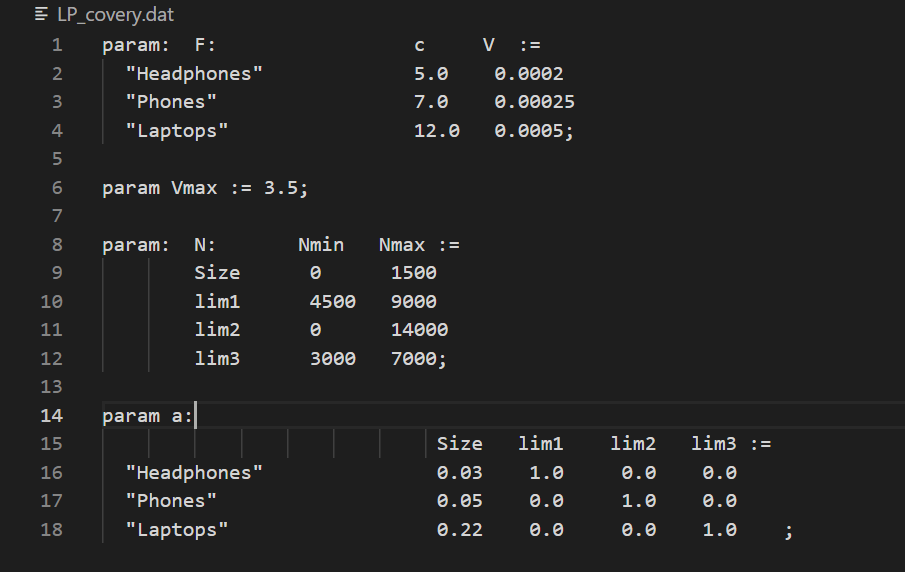
\includegraphics[scale=0.6]{pictures/task_11_ydat.png} \\
    data for linear programming in terms of y
\end{center}

\begin{center}
    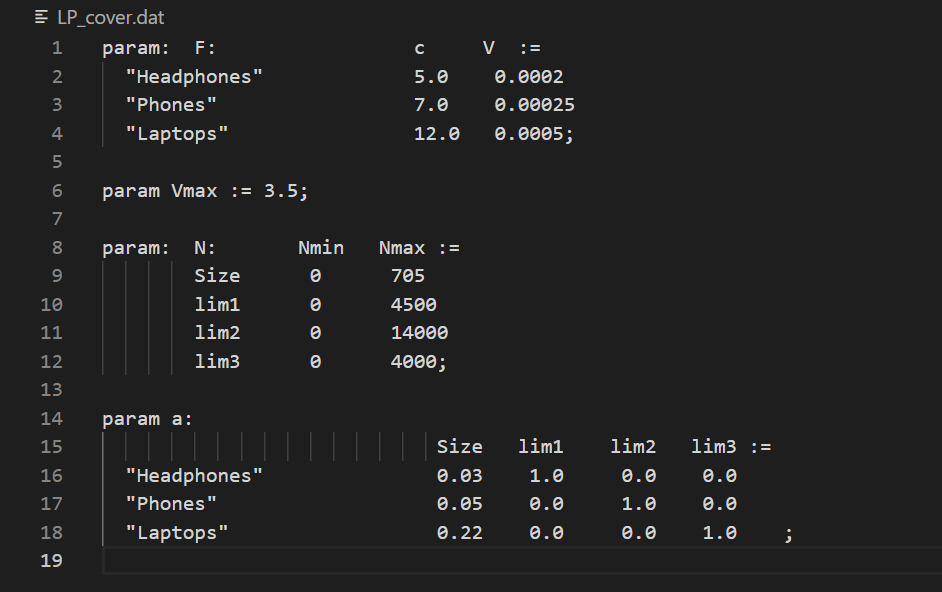
\includegraphics[scale=0.6]{pictures/task_11_xdat.png} \\
    data for linear programming in terms of x
\end{center}

\begin{center}
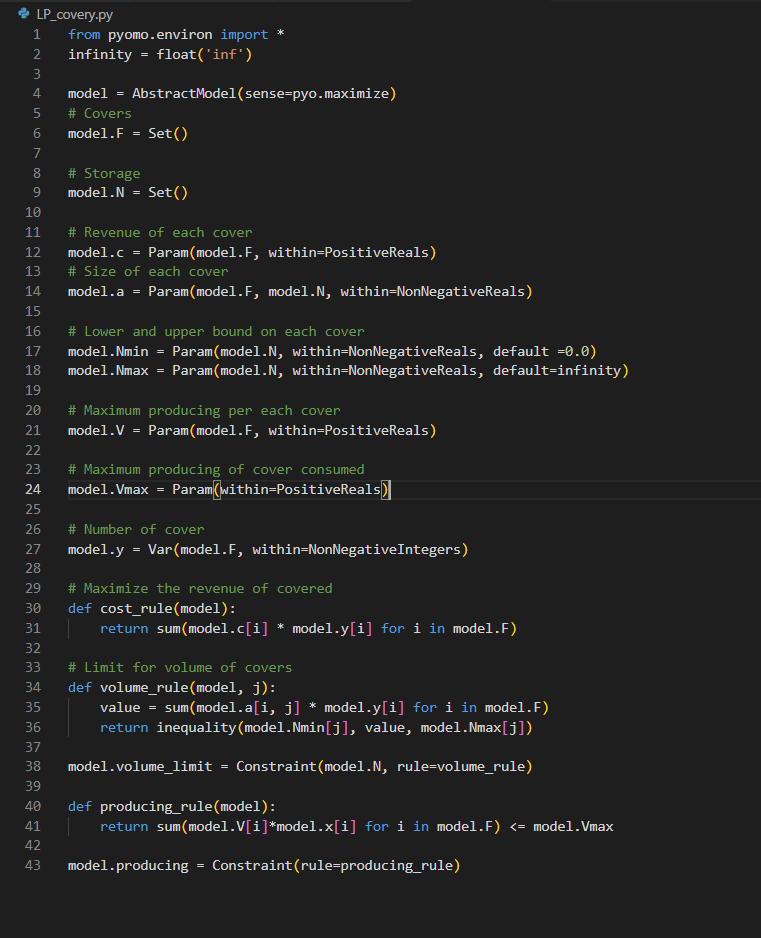
\includegraphics[scale=0.9]{pictures/task_11_ypy.png} \\
solutions in terms of y
\end{center}

\begin{center}
    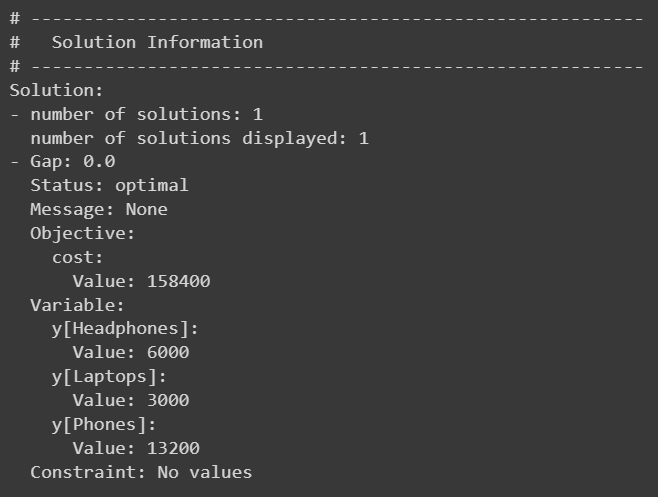
\includegraphics[scale=0.58]{pictures/task_11_yans.png} \\
    answer problem in terms of y
\end{center}

\begin{center}
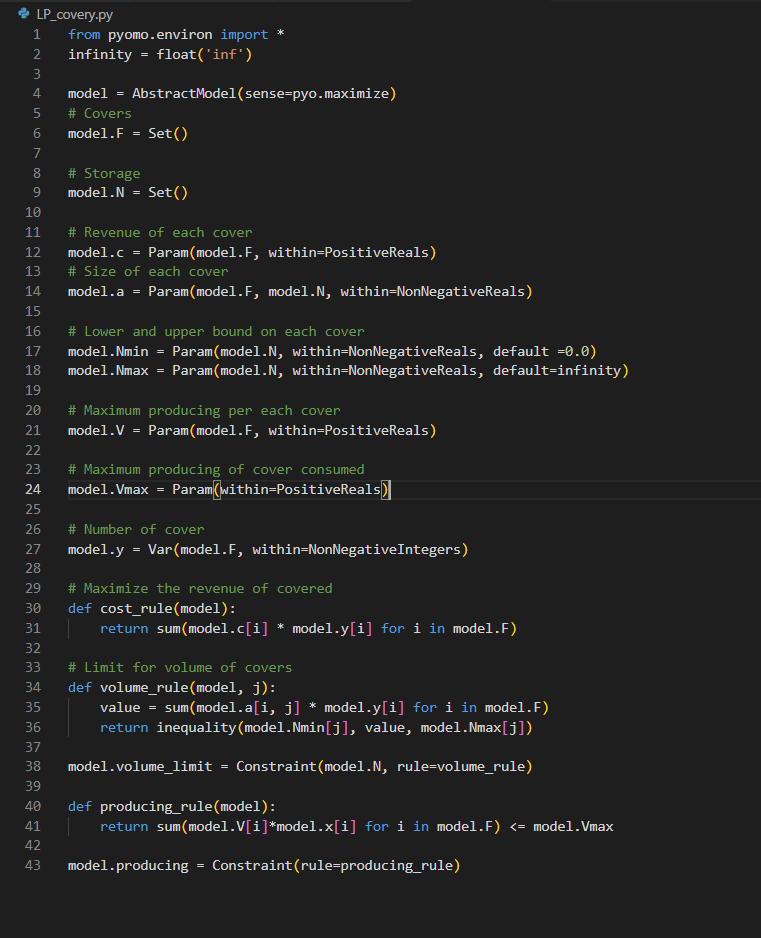
\includegraphics[scale=0.9]{pictures/task_11_xpy.png} \\
solutions in terms of x
\end{center}

\begin{center}
    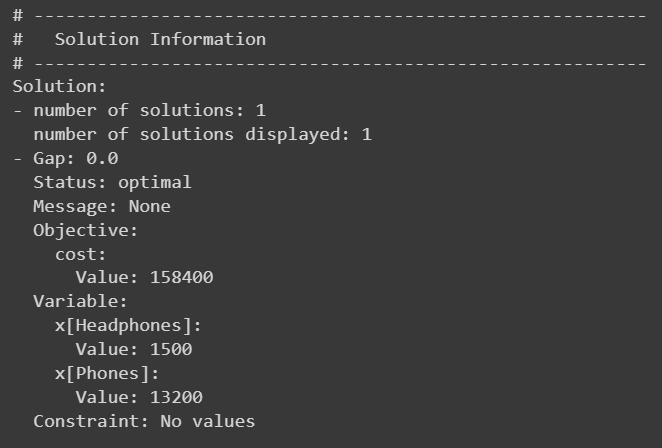
\includegraphics[scale=0.58]{pictures/task_11_xans.png} \\
    answer problem in terms of x
\end{center}


\subsection{Problem №2}
Prove the optimality of the solution
\begin{equation*}
    x^T = \left( \frac{5}{26}, \frac{5}{2}, \frac{27}{26} \right)
\end{equation*}

to the following linear programming problem:
\begin{equation*}
    9x_1 + 14x_2 + 7x_3 \rightarrow \max_{x \in \mathds{R}^n}
\end{equation*}

\begin{equation*}
\begin{gathered}
    \text{s.t. } 2x_1 + x_2 + 3x_3 \leq 6 \\
    5x_1 + 4x_2 + x_3 \leq 12 \\
    2x_2 \leq 5
\end{gathered}
\end{equation*}
buy you cannot use any numerical algorithm here.

\underline{\textbf{Solution:}}
Point $x = \left( 0, 0, 0 \right)^T$ satisfies Slater's conditions.

\begin{equation*}
\begin{gathered}
        0 < 6  \\
        0 < 12 \\
        0 < 5
\end{gathered}
\end{equation*}
And KKT becomes necessary and sufficient.

\begin{equation*}
    L(x, \lambda) = 9x_1 + 14x_2 + 7x_3 - \lambda_1(2x_1 + x_2 + 3x_3 - 6) - \lambda_2(5x_1 + 4x_2 + x_3 - 12) - \lambda_3 (2x_2 -5)
\end{equation*}

\begin{equation*}
    \begin{cases}
    \nabla_{x_1} L = 9  - 2\lambda_1 - 5\lambda_2 = 0 \\
    \nabla_{x_2} L = 14 - \lambda_1  - 4\lambda_2 - 2\lambda_3 = 0 \\
    \nabla_{x_3} L = 7  - 3\lambda_1 - \lambda_2 = 0 \\
    \lambda \succcurlyeq 0 \\
    \lambda_1 (2x_1 + x_2 + 3x_3 - 6) = 0 \\
    \lambda_2 (5x_1 + 4x_2 + x_3 - 12) = 0 \\
    \lambda_3 (2x_2 - 5) = 0 \\
    2x_1 + x_2 + 3x_3 \leq 6 \\
    5x_1 + 4x_2 + x_3 \leq 12 \\
    2x_2 \leq 5
    \end{cases}
\end{equation*}
From it we get:
\begin{equation*}
\begin{cases}
    \lambda_1 = 2 \\
    \lambda_2 = 1 \\
    \lambda_3 = 4 \\
    \lambda \succcurlyeq 0 \\
    2\cdot(2 \cdot \frac{5}{26} + \frac{5}{2} + 3 \cdot \frac{27}{27} - 6) = 2\cdot(6 -6) = 0 \\
    1 \cdot(5 \cdot \frac{5}{26} + 4 \cdot \frac{5}{2} + \frac{27}{27} - 12) = 12 - 12 = 0 \\
    4 \cdot (2 \frac{5}{2} - 5) = 0 \\
    2 \cdot \frac{5}{26} + \frac{5}{2} + 3 \cdot \frac{27}{27} = 6 \leq 6 \\  
    5 \cdot \frac{5}{26} + 4 \cdot \frac{5}{2} + \frac{27}{27} = 12 \leq 12 \\
    2 \frac{5}{2} = 5 \leq 5
\end{cases}
\end{equation*}
\begin{equation*}
    L(\frac{5}{26}, \frac{5}{2}, \frac{27}{26}) = 9 \cdot \frac{5}{26} + 14 \frac{5}{2} + 7 \frac{27}{26} - 2 \cdot(6-6) - (12 - 12) - 4 \cdot (5 - 5) = \frac{45 + 70 + 189}{26} = \frac{304}{26}
\end{equation*}
Optimal point: $\frac{152}{13}$

We show that this problem satisfies Slater's conditions and KKT becomes essential and suffiecient condition. And point $x = \left( \frac{5}{26}, \frac{5}{2}, \frac{27}{26} \right)^T$ satisfies the conditions of the KKT.

\subsection{Problem №3}
Transform the following linear program into an equivalent linear programm in standart form($c^Tx \rightarrow \max_{x \in \mathds{R}^n} : Ax = b, x \geq 0$):


\begin{equation*}
    x_1 - x_2 \rightarrow \min_{x \in \mathds{R}^n}
\end{equation*}

\begin{equation*}
\begin{gathered}
    \text{s.t. } 2x_1 + x_2 \geq 3 \\
    3x_1 - x_2 \leq 7 \\
    x_1 \geq 0
\end{gathered}
\end{equation*}

\underline{\textbf{Solution:}}

Let's take $x_1 = x$, $X_2 = y - z$, where $y = x_{2+}$, $z = x_{2-}$, $y, z \geq 0$
And rewrite our problem.

\begin{equation*}
    x_1 - x_2 \rightarrow \min_{x \in \mathds{R}^3}
\end{equation*}

\begin{equation*}
\begin{gathered}
    \text{s.t. } -2x_1 - y + z \leq 3 \\
    3x_1 - y + z \leq 7 \\
    x_1 \geq 0 \\
    y \geq 0 \\
    z \geq 0
\end{gathered}
\end{equation*}
Okay, let's again rewrite it.

\begin{equation*}
    x - y + z \rightarrow \min_{x \in \mathds{R}^3}
\end{equation*}

\begin{equation*}
\begin{gathered}
    \text{s.t. } 
    \begin{pmatrix}
    2  & 1  & -1 \\
    3  & -1 & 1 \\
    -1 & 0  & 0 \\
    0  & -1 & 0 \\
    0  & 0  & -1 
    \end{pmatrix} 
    \begin{bmatrix}
    x \\
    y \\
    z
    \end{bmatrix} \succcurlyeq \begin{pmatrix}
        3 \\
        3 \\
        0 \\
        0 \\
        0
    \end{pmatrix} 
\end{gathered}
\end{equation*}
But we need to rewrite it standart form, not it's canonical form.

\begin{equation*}
\begin{gathered}
    c = \left(1, -1, 0\right)^T \\
    A = \begin{pmatrix}
    2  & 1  & -1 \\
    3  & -1 & 1 \\
    -1 & 0  & 0 \\
    0  & -1 & 0 \\
    0  & 0  & -1 
    \end{pmatrix} \\
    b = \left(3, 3, 0, 0, 0\right)^T
\end{gathered}
\end{equation*}

\begin{equation*}
    L(x, \lambda) = c^Tx + \lambda^T(Ax - b) = (c^T + \lambda^TA-)x - \lambda^T b
\end{equation*}
\begin{equation*}
    g(\lambda) = \inf_{x \in \mathds{R}^3} \left(c^T + \lambda^TA \right)x - \lambda^T b
\end{equation*}

And we have: 
\begin{equation*}
    -b^T\lambda\rightarrow \max_{\lambda \in \mathds{R}^5}
\end{equation*}

\begin{equation*}
\begin{gathered}
    \text{s.t. } A^T\lambda = - c \\
    \lambda \succcurlyeq 0
\end{gathered}
\end{equation*}

And finally:
\begin{equation*}
    -\left(3, 3, 0, 0, 0 \right)^T\lambda\rightarrow \max_{\lambda \in \mathds{R}^5}
\end{equation*}
\begin{equation*}
\begin{gathered}
    \text{s.t. } \begin{pmatrix}
    2  & 3  & -1 & 0  & 0  \\
    1  & -1 & 0  & -1 & 0  \\
    -1 & 1  & 0  & 0  & -1 \\
    \end{pmatrix} \lambda = (-1, 1, 0)^T \\
    \lambda \succcurlyeq 0
\end{gathered}
\end{equation*}

\subsection{Problem №4}
Consider
\begin{equation*}
    4x_1 + 5x_2 + 2x_3 \rightarrow \max_{x \in \mathds{R}^3}
\end{equation*}
\begin{equation*}
\begin{gathered}
    \text{s.t. } 2x_1 - x_2 + 2x_3 \leq 9 \\
    3x_1 + 5x_2 + 4x_3 \leq 8 \\
    x_1 + x_2 + 2x_3 \leq 2 \\
    x_1, x_2, x_3 \geq 0
\end{gathered}
\end{equation*}
\begin{enumerate}
    \item[a] Find an optimal solution to the Linear Programming using the simplex method.
    \item[b] Write the dual linear program. Find an optimal dual solution. Do we have strong duality here?
\end{enumerate}

\underline{\textbf{Solution:}}
Let's rewrite problem to normal canonical form (by scheme from lecture): 
\begin{equation*}
    \begin{gathered}
        4x_1 + 5x_2 + 2x_3 - x_7 - x_8 - x_9  \rightarrow \max_{x \in \mathds{R}^9}\\
        \text{s.t.  } 2x_1 - x_2 + 2x_3 + x_4 + x_7 = 9\\
                     3x_1 + 5x_2 + 4x_3 + 4x_4 + x_5 + x_8 = 8 \\
                     x_1 + x_2 + x_3 + x_6 + x_9 = 2 \\
                     x_1, x_2, x_3, x_4, x_5, x_6, x_7, x_8, x_9 \geq 0 
    \end{gathered}
\end{equation*}
$4x_1 + 5x_2 + 5x$

First table of simplex method:
\begin{table}[H]
\begin{tabular}{|l|l|l|l|l|l|l|l|l|l|l|l|l|}
\hline
      & c* &    & 0  & 0  & 0  & 0  & 0  & 0  & -1 & -1 & -1 &     \\ \hline
Basis &    & b   & a1 & a2 & a3 & a4 & a5 & a6 & a7 & a8 & a9 & t   \\ \hline
a7    & -1 & 9   & 2  & -1 & 2  & 1  & 0  & 0  & 1  & 0  & 0  & 4.5 \\ \hline
a8    & -1 & 8   & 3  & 5  & 4  & 0  & 1  & 0  & 0  & 1  & 0  & 2   \\ \hline
a9    & -1 & 2   & 1  & 1  & 2  & 0  & 0  & 1  & 0  & 0  & 1  & 1   \\ \hline
z     &    & -19 & -6 & -5 & -8 & -1 & -1 & -1 & -1 & -1 & -1 &     \\ \hline
delta &    &     & -6 & -5 & -8 & -1 & -1 & -1 & 0  & 0  & 0  &     \\ \hline
\end{tabular}
\end{table}

New basis: $a_3, a_7, a_8$.

\begin{table}[H]
\begin{tabular}{|l|l|l|l|l|l|l|l|l|l|l|l|l|}
\hline
      & c* &     & 0   & 0   & 0  & 0  & 0  & 0   & -1 & -1 & -1  &   \\ \hline
Basis &    & b   & a1  & a2  & a3 & a4 & a5 & a6  & a7 & a8 & a9  & t \\ \hline
a3    & 0  & 1   & 0.5 & 0.5 & 1  & 0  & 0  & 0.5 & 0  & 0  & 0.5 & 2 \\ \hline
a7    & -1 & 7   & 1   & -2  & 0  & 1  & 0  & -1  & 1  & 0  & -1  & 7 \\ \hline
a8    & -1 & 4   & 1   & 3   & 0  & 0  & 1  & 2   & 0  & 1  & 2   & 4 \\ \hline
z     &    & -11 & -2  & -1  & 0  & -1 & -1 & -1  & -1 & -1 & -1  &   \\ \hline
delta &    &     & -2  & -1  & 0  & -1 & -1 & -1  & 0  & 0  & 0   &   \\ \hline
\end{tabular}
\end{table}

New basis: $a_1, a_7, a_8$

\begin{table}[H]
\begin{tabular}{|l|l|l|l|l|l|l|l|l|l|l|l|l|}
\hline
      & c* &    & 0  & 0  & 0  & 0  & 0  & 0  & -1 & -1 & -1 &     \\ \hline
Basis &    & b  & a1 & a2 & a3 & a4 & a5 & a6 & a7 & a8 & a9 & t   \\ \hline
a1    & 0  & 2  & 1  & 1  & 2  & 0  & 0  & 1  & 0  & 0  & 1  & --- \\ \hline
a7    & -1 & 5  & 0  & -3 & -2 & 1  & 0  & -2 & 1  & 0  & -2 & 5   \\ \hline
a8    & -1 & 2  & 0  & 2  & 2  & 0  & 1  & -3 & 0  & 1  & -3 & --- \\ \hline
z     &    & -7 & 0  & 1  & 0  & -1 & -1 & 5  & -1 & -1 & 5  &     \\ \hline
delta &    &    & 0  & 1  & 0  & -1 & -1 & 5  & 0  & 0  & 6  &     \\ \hline
\end{tabular}
\end{table}

New basis: $a_1, a_7, a_5$.
\begin{table}[H]
\begin{tabular}{|l|l|l|l|l|l|l|l|l|l|l|l|l|}
\hline
      & c* &    & 0  & 0  & 0  & 0  & 0  & 0  & -1 & -1 & -1 &    \\ \hline
Basis &    & b  & a1 & a2 & a3 & a4 & a5 & a6 & a7 & a8 & a9 & t  \\ \hline
a1    & 0  & 2  & 1  & 1  & 2  & 0  & 0  & 1  & 0  & 0  & 1  & -- \\ \hline
a7    & -1 & 5  & 0  & -3 & -2 & 1  & 0  & -2 & 1  & 0  & -2 & 5  \\ \hline
a5    & 0  & 2  & 0  & 2  & 2  & 0  & 1  & -3 & 0  & 1  & -3 & -- \\ \hline
z     &    & -5 & 0  & 3  & 2  & -1 & 0  & 2  & -1 & 0  & 2  &    \\ \hline
delta &    &    & 0  & 3  & 2  & -1 & 0  & 2  & 0  & 1  & 3  &    \\ \hline
\end{tabular}
\end{table}

New basis: $a_1, a_4, a_5$.

\begin{table}[H]
\begin{tabular}{|l|l|l|l|l|l|l|l|l|l|l|l|l|}
\hline
      & c* &   & 0  & 0  & 0  & 0  & 0  & 0  & -1 & -1 & -1 &   \\ \hline
Basis &    & b & a1 & a2 & a3 & a4 & a5 & a6 & a7 & a8 & a9 & t \\ \hline
a1    & 0  & 2 & 1  & 1  & 2  & 0  & 0  & 1  & 0  & 0  & 1  &   \\ \hline
a4    & 0  & 5 & 0  & -3 & -2 & 1  & 0  & -2 & 1  & 0  & -2 &   \\ \hline
a5    & 0  & 2 & 0  & 2  & -2 & 0  & 1  & -3 & 0  & 1  & -3 &   \\ \hline
z     &    & 0 & 0  & 0  & 0  & 0  & 0  & 0  & 0  & 0  & 0  &   \\ \hline
delta &    &   & 0  & 0  & 0  & 0  & 0  & 0  & 1  & 1  & 1  &   \\ \hline
\end{tabular}
\end{table}
$\Delta \geq 0$, from that we get $x = (2, 0, 0, 5, 2, 0, 0, 0, 0)^T$ - solution of this problem.

Extreme point for the original problem will be: $x = (2, 0, 0, 5, 2, 0)^T$.

Solution of the original problem.

\begin{table}[H]
\begin{tabular}{|l|l|l|l|l|l|l|l|l|l|}
\hline
      & c* &   & 4  & 5  & 2  & 0  & 0  & 0  &   \\ \hline
Basis &    & b & a1 & a2 & a3 & a4 & a5 & a6 & t \\ \hline
a1    & 4  & 2 & 1  & 1  & 2  & 0  & 0  & 1  & 2 \\ \hline
a4    & 0  & 5 & 0  & -3 & -2 & 1  & 0  & -2 &   \\ \hline
a5    & 0  & 2 & 0  & 2  & 2  & 0  & 1  & -3 & 1 \\ \hline
z     &    & 8 & 4  & 4  & 8  & 0  & 0  & 4  &   \\ \hline
delta &    &   & 0  & -1 & 6  & 0  & 0  & 4  &   \\ \hline
\end{tabular}
\end{table}

New basis: $a_1, a_2, a_5$.

\begin{table}[H]
\begin{tabular}{|l|l|l|l|l|l|l|l|l|l|}
\hline
      & c* &   & 4  & 5  & 2  & 0  & 0    & 0    &   \\ \hline
Basis &    & b & a1 & a2 & a3 & a4 & a5   & a6   & t \\ \hline
a1    & 4  & 1 & 1  & 0  & 3  & 0  & -0.5 & 2.5  &   \\ \hline
a2    & 5  & 1 & 0  & 1  & -1 & 0  & 0.5  & -1.5 &   \\ \hline
a4    & 0  & 8 & 0  & 0  & -5 & 1  & 1.5  & -6.5 &   \\ \hline
z     &    & 9 & 4  & 5  & 7  & 0  & 0.5  & 2.5  &   \\ \hline
delta &    &   & 0  & 0  & 5  & 0  & 0.5  & 2.5  &   \\ \hline
\end{tabular}
\end{table}

Solution is $(1, 1, 0, 8, 0, 0)^T$. Comeback to our original problem, get rid of 3 latest coordinates, point will be: $(1, 1, 0)^T$ on that point maximum will be achieve. Maximum equals 9.

\underline{\textbf{Answer:}} maximum equals 9, in point $x = (1, 1, 0)^T$.

\underline{\textbf{Solution:}}
\begin{equation*}
\begin{gathered}
    L(x, \lambda) = 4x_1 + 5x_2 + 2x_3 - \lambda_1(2x_1 - x_2 + 2x_3 -9) - \lambda_2(3x_1 + 5x_2 + 4x_3 -8) \\
    - \lambda_3(x_1 + x_2 + 2x_3 -2) + \lambda_4 x_1 + \lambda_5 x_2 + \lambda_6 x_3
\end{gathered}
\end{equation*}

Slater's conditins met and KKT conditions are necessary and sufficient.

\begin{equation*}
    \begin{cases}
    \nabla_{x_1} L = 4  - 2\lambda_1 - 3\lambda_2 - \lambda_3 + \lambda_4 = 0 \\
    \nabla_{x_2} L = 5  + 1\lambda_1  - 5\lambda_2 - \lambda_3 + \lambda_5 = 0 \\
    \nabla_{x_3} L = 2  - 2\lambda_1 - 4\lambda_2 - 2\lambda_3 + \lambda_6 = 0 \\
    
    \lambda \succcurlyeq 0 \\
    \lambda_1 (2x_1 - x_2 + 2x_3 - 9) = 0 \\
    \lambda_2 (x_1 + 5x_2 + 4x_3 - 8) = 0 \\
    \lambda_3 (x_1 + x_2 + 2x_3 - 2) = 0 \\
    \lambda_4 x_1 = 0 \\
    \lambda_5 x_2 = 0 \\
    \lambda_6 x_3 = 0 \\
    2x_1 - x_2 + 2x_3 \leq 9 \\
    3x_1 + 5x_2 + 4x_3 \leq 8 \\
    x_1 + x_2 + 2x_3 \leq 2 \\
    x_1, x_2, x_3 \geq 0
    \end{cases}
\end{equation*}


We have strong duality because KKT conditions are necessary and sufficient. 
Point $x^* = (1, 1, 0)^T$ is feasible for that. 
